\documentclass{article}

\usepackage{amsmath}
\usepackage{amsthm}
\usepackage{amssymb}

\usepackage[margin=1.8cm]{geometry}
\usepackage{tikz}

\begin{document}

\section*{Convergent Circle Corners}

\subsection*{Circle Areas}

Given two points on the first quadrant of unit circle \( A, B \), we may define
a new unique point \( C = A \oplus B \) through the following: extend a
horizontal line through the \( y \)-coordinate of the point with the smaller \(
x \)-coordinate. Next, extend a vertical line through the \( x \)-coordinate of
the point with the larger \( x \)-coordinate. Find the point of intersection
between these two lines and draw a line with slope \( 1 \) running through this
point. The new point \( C \) shall be the intersection of this line with the
unit circle in the first quadrant.

More explicitly, suppose that \( A = \left( x_1, y_1 \right), B = \left( x_2,
y_2 \right), x_1 \leqslant x_2 \). Then we have that
\[
    C = \left( \frac{x_2 - y_1 + \sqrt{2 - \left( x_2 - y_1 \right)^2}}{2}, \frac{y_1 - x_2 + \sqrt{2 - \left( y_1 - x_2 \right)^2}}{2} \right)
.\]

% Lol the figure looks kinda wonky but it'll do for now I guess
\begin{center}
\begin{tikzpicture}[scale=4]
    \draw (1, 0) arc (0:90:1);
    \draw[->] (-0.05, 0) -- (1.2, 0);
    \draw[->] (0, -0.05) -- (0, 1.2);

    \node (A) at ({cos(75)}, {sin(75)}) {};
    \node[anchor=south] at (A) {A};
    \fill (A) circle (0.012);

    \node (B) at ({cos(30)}, {sin(30)}) {};
    \node[anchor=west] at (B) {B};
    \fill (B) circle (0.012);

    \draw[->] ({cos(75)}, {sin(75)}) -- ({cos(75) + 1}, {sin(75)});
    \draw[->] ({cos(30)}, {sin(30)}) -- ({cos(30)}, {sin(30) + 0.7});
    \draw[->] ({cos(30) + 0.02}, {sin(75) + 0.02}) -- ({cos(30) - 0.5}, {sin(75) - 0.5});

    \node (C) at (0.655390115, 0.75529053) {};
    \node[anchor=north] at (C) {C};
    \fill (C) circle (0.012);
\end{tikzpicture}
\end{center}

With this, we can begin to build up our circle corner converging series. We can
build this recursively, starting with an initial condition. For \( n \geqslant
0 \), define \( S_n \) to be the ordered set (according to \( x \)-coordinate)
of all corner points lying on the unit circle quadrant. We let \( S_0 = \left(
\left( 0, 1 \right), \left( 1, 0 \right) \right) \) to start with and then use
the following recursive definition: suppose \( S_n = \left( P_1, P_2, \ldots,
P_k \right) \); we have
\[
    S_{n+1} = \left( P_1, P_1 \oplus P_2, P_2, \ldots, P_{k-1}, P_{k - 1} \oplus P_k, P_k \right)
.\]
% Ok I fixed it
% (Actually, I'm now doubting that this is in fact true, considering that we only
% really want to find the corners between neighboring points and not all of
% them. The fact that the sum seems to move towards \( \pi \) for increasing
% values of \( n \) isn't really too much indication that things are going right
% as the Darboux integral of any decently well-behaved partition of \( \left[ 0,
% 1 \right] \) will likely approach the Riemann integral, and give us our value
% of \( \pi \). Certainly the operation we have is correct, but I don't think
% building the set recursively is as easy as this).
One can confirm that for \( n \geqslant 1 \), there are \( k = 2^n + 1 \) points in
\( S_n \).

We now desire the area of the converging corners shape. Fix a specific \( n \)
and look at the ordered set of points \( S_n = \left( \left( x_1, y_1 \right),
\left( x_2, y_2 \right), \ldots, \left( x_k, y_k \right) \right) \). We then
have that the total area is
\[
    A_n = 4 \sum_{i = 1}^{k - 1} y_i \left( x_{i + 1} - x_i \right)
.\]
We assert that this area approaches \( \pi \) as \( n \to \infty \), but I
can't properly show this right now.

Now that we have mathematically formulated this, perhaps it would be a good
exercise to code it. As for how to formally show that this approaches \( \pi
\), I'll have to think about it (and perhaps try a different approach). For
now, it will do good to verify it empirically though. Certainly the previous
series looks suspiciously like an integral (in fact it is called the Darboux
integral), so perhaps our proof shall rely upon this.

In coding a rough example, we can see empirically that the area does roughly
approach \( \pi \), albeit a bit slowly considering the number of points. We have
\begin{center}
\begin{tabular}{c|c|c}
    \( n \) & Points & Area \\
    \hline
    1 & 3 & 3.6568542494923806\\
    2 & 5 &  3.447477652576853 \\
    3 & 9 &  3.324791968290031 \\
    4 & 17 & 3.2536764558450173 \\
    5 & 33 & 3.2121295100035105 \\
    \vdots & \vdots & \vdots \\
    20 & 1048577 & 3.1430271877389186 
\end{tabular}
\end{center}
I'm not quite sure how to express a good closed form for any of this, but
certainly we can prove that the maximum difference between the \( x \)
coordinates of the points goes to \( 0 \), but I'm not sure whether this is any
help for proving that the Darboux integral approaches the Riemann integral or
anything of the sort.

\vspace{0.5cm}

\begin{center}
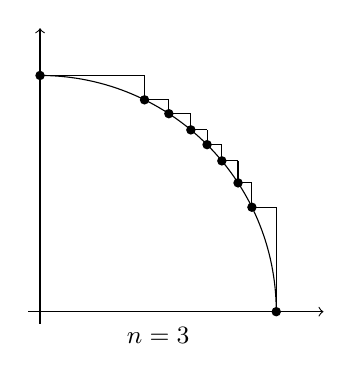
\begin{tikzpicture}[scale=3]
    \draw (1, 0) arc (0:90:1);
    \draw[->] (-0.05, 0) -- (1.2, 0);
    \draw[->] (0, -0.05) -- (0, 1.2);

    \node at (0.5, -0.1) {\small \( n = 3 \)};

    \foreach \point in {(0, 1), (0.44223040680405135, 0.8969014813779289), (0.5453289254261224, 0.8382221442395749), (0.6385035305799822, 0.7696188936330095), (0.7071067811865476, 0.7071067811865476), (0.7696188936330095, 0.6385035305799823), (0.8382221442395748, 0.5453289254261223), (0.8969014813779288, 0.4422304068040511), (1, 0)} {
        \fill \point circle (0.02);
    }

    \draw (0, 1) -- (0.44223040680405135, 1);
    \draw (0.44223040680405135, 1) -- (0.44223040680405135, 0.8969014813779289);
    \draw (0.44223040680405135, 0.8969014813779289) -- (0.5453289254261224, 0.8969014813779289);
    \draw (0.5453289254261224, 0.8969014813779289) -- (0.5453289254261224, 0.8382221442395749);
    \draw (0.5453289254261224, 0.8382221442395749) -- (0.6385035305799822, 0.8382221442395749);
    \draw (0.6385035305799822, 0.8382221442395749) -- (0.6385035305799822, 0.7696188936330095);
    \draw (0.6385035305799822, 0.7696188936330095) -- (0.7071067811865476, 0.7696188936330095);
    \draw (0.7071067811865476, 0.7696188936330095) -- (0.7071067811865476, 0.7071067811865476);
    \draw (0.7071067811865476, 0.7071067811865476) -- (0.7696188936330095, 0.7071067811865476);
    \draw (0.7696188936330095, 0.7071067811865476) -- (0.7696188936330095, 0.6385035305799823);
    \draw (0.7696188936330095, 0.6385035305799823) -- (0.8382221442395748, 0.6385035305799823);
    \draw (0.8382221442395748, 0.6385035305799823) -- (0.8382221442395748, 0.5453289254261223);
    \draw (0.8382221442395748, 0.5453289254261223) -- (0.8969014813779288, 0.5453289254261223);
    \draw (0.8969014813779288, 0.5453289254261223) -- (0.8969014813779288, 0.4422304068040511);
    \draw (0.8969014813779288, 0.4422304068040511) -- (1, 0.4422304068040511);
    \draw (1, 0.4422304068040511) -- (1, 0);
\end{tikzpicture}
\end{center}

\subsection*{Darboux goes to Riemann?}

The quickest explanation of the Darboux integral is that it is equivalent to
the definition of a Riemann integral except for the fact that the \( x \)
differences between each point don't necessarily have to be equal. We instead
define a partition of the interval that we're integrating over and tile this
interval with not necessary equal lengths. In practice, this makes them easier
to work with in real analysis to prove whether things are Riemann integrable,
but we're using them for a slightly different purpose it seems.

As for whether the values of Darboux integrals and Riemann integrals converge
to each other as \( n \to \infty \), it's a bit hard to say. Intuitively, one
would think that they would, but this isn't the first time that real analysis
has Looney Tooned people, so I'm going to be a bit wary. Wikipedia was a bit
vague in stating this fact as well, with the citation coming from a large real
analysis textbook that might be a bit above my pay grade, so we're going to do
some street mathematics.

In order to satisfy me that these two sums are equal, I'm going to see what the
ratio of the maximum \( x \) distance and the mininum \( x \) distance in the
partition at \( n \to \infty \) looks like. Supposing that the ratio is \( 1
\), one could use the sandwich theorem to then assert that all the distances
would be equal, thus giving us a Riemann integral. So now all that's left to
determine is this ratio.

I state without much formal proof that the maximum \( x \) difference found in
our partition is found between the first and second points in the partition.
This one perhaps makes a bit of intuitive sense due to how the points are
spread out.

\begin{center}
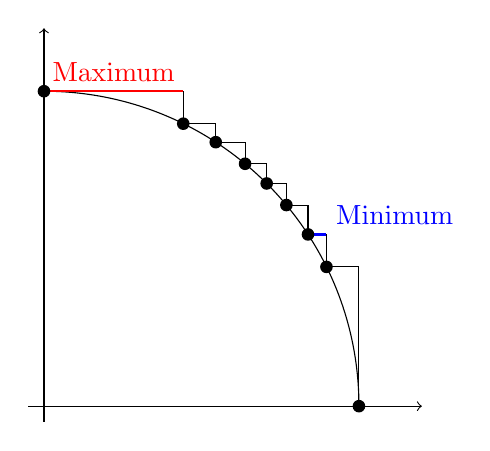
\begin{tikzpicture}[scale=4]
    \draw (1, 0) arc (0:90:1);
    \draw[->] (-0.05, 0) -- (1.2, 0);
    \draw[->] (0, -0.05) -- (0, 1.2);

    \draw[red, thick] (0, 1) -- (0.44223040680405135, 1);
    \node[red, anchor=south] at (0.44223040680405135 / 2, 1) {Maximum};
    \draw (0.44223040680405135, 1) -- (0.44223040680405135, 0.8969014813779289);
    \draw (0.44223040680405135, 0.8969014813779289) -- (0.5453289254261224, 0.8969014813779289);
    \draw (0.5453289254261224, 0.8969014813779289) -- (0.5453289254261224, 0.8382221442395749);
    \draw (0.5453289254261224, 0.8382221442395749) -- (0.6385035305799822, 0.8382221442395749);
    \draw (0.6385035305799822, 0.8382221442395749) -- (0.6385035305799822, 0.7696188936330095);
    \draw (0.6385035305799822, 0.7696188936330095) -- (0.7071067811865476, 0.7696188936330095);
    \draw (0.7071067811865476, 0.7696188936330095) -- (0.7071067811865476, 0.7071067811865476);
    \draw (0.7071067811865476, 0.7071067811865476) -- (0.7696188936330095, 0.7071067811865476);
    \draw (0.7696188936330095, 0.7071067811865476) -- (0.7696188936330095, 0.6385035305799823);
    \draw (0.7696188936330095, 0.6385035305799823) -- (0.8382221442395748, 0.6385035305799823);
    \draw (0.8382221442395748, 0.6385035305799823) -- (0.8382221442395748, 0.5453289254261223);
    \draw[blue, thick] (0.8382221442395748, 0.5453289254261223) -- (0.8969014813779288, 0.5453289254261223);
    \node[blue, anchor=south west] at (0.8969014813779288, 0.5453289254261223) {Minimum};
    \draw (0.8969014813779288, 0.5453289254261223) -- (0.8969014813779288, 0.4422304068040511);
    \draw (0.8969014813779288, 0.4422304068040511) -- (1, 0.4422304068040511);
    \draw (1, 0.4422304068040511) -- (1, 0);

    \foreach \point in {(0, 1), (0.44223040680405135, 0.8969014813779289), (0.5453289254261224, 0.8382221442395749), (0.6385035305799822, 0.7696188936330095), (0.7071067811865476, 0.7071067811865476), (0.7696188936330095, 0.6385035305799823), (0.8382221442395748, 0.5453289254261223), (0.8969014813779288, 0.4422304068040511), (1, 0)} {
        \fill \point circle (0.02);
    }
\end{tikzpicture}
\end{center}

The minimum case is a bit more wacky, and I had to test it out empirically to
find out whether there was a real pattern. Doing so, one can build the following table for \( n \).

\begin{center}
\begin{tabular}{c|c}
    \( n \) & Index of Min \\
    \hline
    1 & 1 \\
    2 & 2 \\
    3 & 6 \\
    4 & 12 \\
    5 & 24 \\
    6 & 56 \\
    7 & 112 \\
    8 & 224 \\
    9 & 448 \\
    10 & 960 \\
    11 & 1920 \\
    12 & 3840 \\
    13 & 7936 \\
    14 & 15872 \\
    15 & 31744 \\
    16 & 63488 \\
    17 & 129024 \\
    18 & 258048 \\
    19 & 516096 \\
    20 & 1040384 \\
\end{tabular}
\end{center}

Every so often (it appears to be when \( n \equiv 3, 6 \pmod{7} \)), the index
of the minimum jumps around, while for the others it simply doubles
(corresponding to the same point as the previous \( n \) given the doubling
nature of the points through each iteration). The size of these jumps appeared
to be powers of \( 8 \), but the \( n = 20 \) case destroys this pattern.

Even if one were to be able to determine the exact index of the minimum, it
seems that it would be quite cumbersome to find the actual minimum length
described by it and the point in front of it, which is really not nice of it.

While we certainly can't do this for the minimum length, we can try it on some
easier to work with lengths. This doesn't really prove a lot (we can't use the
same sandwich theorem consequence really), but it seems to be the only way to
proceed from here, so it might help to try it. As such, pick our ``minimum'' to
be the distance between the exact middle point (which is at \( \left(
\cos{\left( \pi/4 \right)}, \sin{\left( \pi/4 \right)} \right) \)) and the
point in front of it. This makes things a bit easier to calculate and work
with.

Denote \( G_n \) the second point in the ordered set. We have the following recursion:
\[
    G_{n + 1} = \left( 0, 1 \right) \oplus G_n
.\]
Something similar follows for our other extreme. Denote \( L_n \) the point after the midway point in the ordered set. We have:
\[
    L_{n + 1} = \left( \frac{1}{\sqrt{2}}, \frac{1}{\sqrt{2}} \right) \oplus L_n
.\]
We can easily extract the extreme lengths now by simply subtracting the \( x \)
coordinates of these points with that of the point directly before them. Let \(
g_n \) denote the \( x \) component of \( G_n \) and \( l_n \) denote the \( x
\) component of \( L_n \) minus \( 1 / \sqrt{2} \). We desire the following
limit:
\[
    \lim_{n \to \infty} \frac{l_n}{g_n}
.\]
Now we must solve the recurrences.

\subsubsection*{Obtaining \( g_n, l_n \)}

Let us use the explicit definition of the ``cornering'' operator. Suppose \( G_n = \left( x_n, y_n \right) \); then
\[
    \left( x_{n + 1}, y_{n + 1} \right) = \left( \frac{x_n - 1 + \sqrt{2 - \left( x_n - 1 \right)^2}}{2}, \frac{1 - x_n + \sqrt{2 - \left( 1 - x_n \right)^2}}{2} \right)
,\]
where \( \left( x_0, y_0 \right) = \left( 1, 0 \right) \) and \( g_n = x_n \).
We may attempt to solve this recurrence as follows:
\begin{align*}
    g_{n+1} &= \frac{1}{\sqrt{2}} \left( \frac{g_n - 1}{\sqrt{2}} \right) + \frac{1}{\sqrt{2}} \sqrt{1 - \left( \frac{g_n - 1}{\sqrt{2}} \right)^2} \\
    \sqrt{2} \sin{\left( \theta_{n+1} \right)} + 1 &= \frac{1}{\sqrt{2}} \sin{\left( \theta_n \right)} + \frac{1}{\sqrt{2}} \cos{\left( \theta_n \right)} \\
    &= \sin{\left( \theta_n + \pi/4 \right)} \\
    \implies \sin{\left( \theta_{n+1} \right)} &= \frac{1}{\sqrt{2}} \left( \sin{\left( \theta_n + \pi/4 \right)} - 1 \right)
,\end{align*}
where on the second line we make the trig substitution \( \sin{\left( \theta_n
\right)} = \left( g_n - 1 \right) / \sqrt{2} \). From here, it's hard to
proceed. The same case happens for when we try to solve for \( l_n \),
unfortunately, so I'm rather at a loss for how to do this. It seems that
proving that the Darboux integral goes to the Riemann integral with this
approach isn't looking quite promising.

\subsubsection*{Empirical Limits}

That's right, we're back to the even more street mathematics called applied
mathematics where mathematical results are as good as true if we see a pattern
in what the funky computer box outputs. This mathematics has gone so much to
the streets, that I would like to affectionately call it gang mathematics.

That being said, the ratio doesn't seem to approach \( 1 \) as \( n \)
increases (in fact, it seems to approach \( 0 \) if anything), which is
certainly rather confusing. Perhaps this may be a consequence of me only being
able to input \( n = 20 \) before the program drastically slows down, but I
can't say for certain.

\subsubsection*{Conclusion to Darboux and Riemann Integrals}

I don't know a whole lot about real analysis, but I guess one has to assume
that this specific Darboux integral value eventually converges onto Riemann
integral value as \( n \to \infty \).

\subsection*{Conclusion}

It seems unlikely that a better closed form will be possible other than the sum
for \( A_n \) (or the integral of \( \sqrt{1-x^2} \) if you truly believe the
sum approaches the integral), but ultimately this view may be a consequence of
how I tackled the problem. There could be some clever trick to reduce the
problem to something easier to solve, but so far I cannot deduce anything of
such likes.

This was quite a cool problem though.

\end{document}
